\documentclass{homework}
\usepackage{booktabs}
\usepackage{subfig}
\captionsetup[subfigure]{labelformat=empty}


\usepackage{tikz}
\usepackage{pgf}
\usetikzlibrary{arrows,arrows.meta,matrix,shapes.geometric}
\usepackage{xcolor}
\definecolor{mgreen}{HTML}{39825a}

\usepackage{amssymb}% http://ctan.org/pkg/amssymb
\usepackage{pifont}% http://ctan.org/pkg/pifont
\newcommand{\cmark}{\ding{51}}%
\newcommand{\xmark}{\ding{55}}%

\usepackage{fancyvrb,newverbs,xcolor}

\definecolor{cverbbg}{gray}{0.93}

\newenvironment{cverbatim}
 {\SaveVerbatim{cverb}}
 {\endSaveVerbatim
  \flushleft\fboxrule=0pt\fboxsep=.5em
  \colorbox{cverbbg}{\BUseVerbatim{cverb}}
  \endflushleft
}
\newenvironment{lcverbatim}
 {\SaveVerbatim{cverb}}
 {\endSaveVerbatim
  \flushleft\fboxrule=0pt\fboxsep=.5em
  \colorbox{cverbbg}{%
    \makebox[\dimexpr\linewidth-2\fboxsep][l]{\BUseVerbatim{cverb}}
  }
  \endflushleft
}

\newcommand{\ctexttt}[1]{\colorbox{cverbbg}{\texttt{#1}}}
\newverbcommand{\cverb}
  {\setbox\verbbox\hbox\bgroup}
  {\egroup\colorbox{cverbbg}{\box\verbbox}}

\title{CIS 571 - Assignment 2}
\author{Ali Hassani}

\begin{document}

\maketitle

\renewcommand{\theenumi}{\alph{enumi}}
\renewcommand{\theenumii}{\roman{enumii}}

\exercise[1]
\subsection{Draw the constraint graph.}
\begin{figure}[h!]
    \centering
    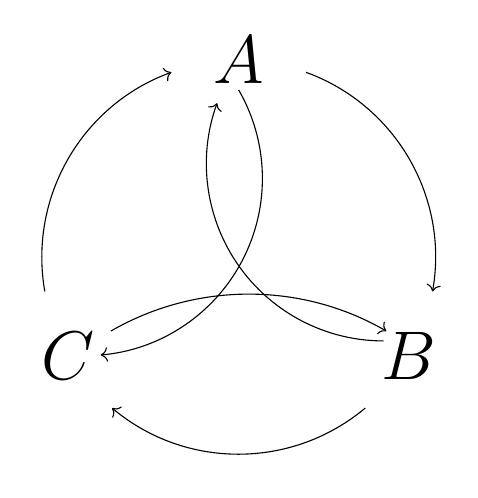
\begin{tikzpicture}[->,scale=2.5]
   \node (A) at (90:1cm)  {\Huge$A$};
   \node (B) at (-30:1cm) {\Huge$B$};
   \node (C) at (210:1cm) {\Huge$C$};

   \draw (70:1cm)  arc (70:-10:1cm);
   \draw (90:0.85cm)  arc (30:-85:0.9cm);
   \draw (-50:1cm) arc (-50:-130:1cm);
   \draw (210:0.75cm)  arc (120:60:1.4cm);
   \draw (190:1cm) arc (190:110:1cm);
   \draw (-30:0.85cm)  arc (270:160:0.9cm);
\end{tikzpicture}

    \caption{Constraint graph}
    \label{fig:q11}
\end{figure}
\subsection{Suppose we are using the AC-3 algorithm for arc consistency. How many total arcs will be en-queued when the algorithm begins execution?}
5 constraints $\Rightarrow$ 10 arcs:
\cverb|(A, B)|, \cverb|(B, A)|, \cverb|(A, C)|, \cverb|(C, A)|, \cverb|(B, C)|, \cverb|(C, B)|, \cverb|(B, D)|, \cverb|(D, B)|, \cverb|(D, C)|, \cverb|(C, D)|.

\subsection{Assuming all ages {8, 9, 10, 11} are possible for each student before running arc consistency, manually run arc consistency on only arc from A to B.}
$d_A = \{8, 9, 10, 11\}$ \\
$ A = 8 \Rightarrow B \in \{10\} $ \cmark \\
$ A = 9 \Rightarrow B \in \{11\} $ \cmark \\
$ A = 10 \Rightarrow B \in \{\} $ \xmark $\quad \Rightarrow d_A = \{8, 9, 11\}$ \\
$ A = 11 \Rightarrow B \in \{\} $ \xmark $\quad\Rightarrow d_A = \{8, 9\}$ \\

\begin{enumerate}
    \item Only $8$ and $9$ remain viable for $A$.
    \item All values technically remain viable, because AC-3 only removes values from the tail domain, and not the head. Therefore, $B$ is not affected.
    \item Neighbors of $A$ would have to be rechecked, which are $B$, $C$ and $D$. Therefore \cverb|(B, A)| \cverb|(C, A)| would be added to the queue.
\end{enumerate}

\subsection{Suppose we enforce arc consistency on all arcs. What ages remain in each person’s domain?}
Assuming \cverb|(A, B)| is already checked ($d_A = \{8, 9\}$):

\cverb|(B, A)|: Values $8$ and $9$ are invalid for $B$, therefore they are removed and \cverb|(A, B)|, \cverb|(C, B)| and \cverb|(D, B)| are added to the queue. $d_B = \{10, 11\}$.

\cverb|(A, C)|: No violations.

\cverb|(C, A)| No violations.

\cverb|(B, C)| No violations.

\cverb|(C, B)| Values $8$ and $9$ are invalid for $C$, therefore they are removed and \cverb|(A, C)|, \cverb|(B, C)| and \cverb|(D, C)| are added to the queue. $d_C = \{10, 11\}$.

\cverb|(B, D)| Value $11$ is invalid for $B$, therefore it is removed and \cverb|(A, B)|, \cverb|(C, B)| and \cverb|(D, B)| are added to the queue. $d_B = \{10\}$.

\cverb|(D, B)| Values $8$, $9$ and $10$ are invalid for $D$, therefore they are removed and \cverb|(A, D)|, \cverb|(B, D)| and \cverb|(C, D)| are added to the queue. $d_D = \{11\}$.

\cverb|(D, C)| No violations.

\cverb|(C, D)| Value $10$ is invalid for $C$, therefore it is removed and \cverb|(A, C)|, \cverb|(B, C)| and \cverb|(D, C)| are added to the queue. $d_C = \{11\}$.

\cverb|(B, A)|, \cverb|(C, A)|: No violations.

\cverb|(A, B)|: Value $9$ is invalid for $A$, therefore it is removed and ... $d_A = \{8\}$. 

Skipping the remaining arcs for simplicity.

Remaining: $d_A = \{8\}$, $d_B = \{10\}$, $d_C = \{11\}$, $d_D = \{11\}$.

\clearpage

\renewcommand{\theenumi}{\arabic{enumi}}

\exercise[2]
\begin{enumerate}
    \item True. Note: technically backtracking is needed, unless arc consistency is set to return a solution if it finds one (every variable can only take 1 value). %1
    \item True. Note: technically backtracking is needed, unless the checking algorithm is set to return a solution if it finds one (every variable can only take 1 value). %2
    \item False %3
    % ?
    \item True %4
    \item False %5
    % 4 nodes, all connected, all have a domain of size 2, ac-3 doesn't eliminate anything.
    \item False %6
    \item True %7
    \item False %8
    \item True %9
    \item False %10
    \item True %11
    \item False %12
    \item True %13
    
\end{enumerate}

\clearpage
\exercise[3]

% \begin{figure}[h!]
%     \centering
%     \includegraphics[width=0.33\textwidth]{figures/3.0.png}
%     \caption{Initial state}
%     \label{fig:q30}
% \end{figure}

\subsection{Step 1}
The random generator selects the left-most of the violating nodes (queens), which are \cverb|Q1|, \cverb|Q2|, and \cverb|Q3|. \cverb|Q4| is not violating any constraints.
\cverb|Q1| is selected, and the number of violations for \cverb|A| through \cverb|D| are 0, 1, 1, 2. Therefore it is moved to \cverb|A|.

% \begin{figure}[h!]
%     \centering
%     \includegraphics[width=0.33\textwidth]{figures/3.1.png}
%     \caption{Step 1}
%     \label{fig:q31}
% \end{figure}

\begin{figure}[h!]
    \centering
    \subfloat[Initial state]{\includegraphics[width=0.33\textwidth]{figures/3.0.png}}
    \qquad
    \subfloat[Step 1]{\includegraphics[width=0.33\textwidth]{figures/3.1.png}}
    \label{fig:q32}
\end{figure}

\subsection{Step 2}
The random generator selects the left-most of the violating nodes (queens), which are \cverb|Q2|, and \cverb|Q3|.
\cverb|Q2| is selected, and the number of violations for \cverb|A| through \cverb|D| are 1, 1, 1, 2. Therefore it is moved to \cverb|A|.

% \begin{figure}[h!]
%     \centering
%     \includegraphics[width=0.33\textwidth]{figures/3.2.png}
%     \caption{Step 2}
%     \label{fig:q32}
% \end{figure}

\begin{figure}[h!]
    \centering
    \subfloat[Step 2]{\includegraphics[width=0.33\textwidth]{figures/3.2.png}}
    \qquad
    \subfloat[Step 3]{\includegraphics[width=0.33\textwidth]{figures/3.3.png}}
    \label{fig:q32}
\end{figure}

\subsection{Step 3}
The random generator selects the left-most of the violating nodes (queens), which are \cverb|Q1|, \cverb|Q2|, and \cverb|Q3|.
\cverb|Q1| is selected, and the number of violations for \cverb|A| through \cverb|D| are 1, 2, 0, 1. Therefore it is moved to \cverb|C|.

\clearpage
\exercise[4]

\subsection{Search}
\subsubsection{Minimax Search}
\begin{figure}[h!]
    \centering
    \input{figures/q41}
    \caption{Minimax Search}
    \label{fig:q41}
\end{figure}
Root node (\cverb|A|) ends up with value 5.

\subsubsection{Alpha-Beta pruning}
\begin{figure}[h!]
    \centering
    
\tikzset{
  regnode/.style = {align=center, inner sep=0pt, text centered,
    font=\sffamily},
  treenode/.style = {align=center, inner sep=0pt, text centered,
    font=\sffamily},
  arn_n/.style = {treenode, circle, white, font=\sffamily\bfseries, draw=black,
    fill=black, text width=1.5em},
  max_n/.style = {regular polygon, regular polygon sides=3, white, font=\sffamily\bfseries, draw=blue, fill=blue},
  max_n_pr/.style = {max_n, draw=gray, gray, fill=white},
  min_n/.style = {regular polygon, regular polygon sides=3, shape border rotate=180, white, font=\sffamily\bfseries, draw=red, fill=red},
  arn_r/.style = {treenode, circle, red, draw=red, 
    text width=1.5em, very thick},
  arn_b/.style = {treenode, circle, blue, draw=blue, 
    text width=1.5em, very thick},
  arn_g/.style = {treenode, circle, white, draw=mgreen, fill=mgreen, 
    text width=1.5em, very thick},
  arn_w/.style = {treenode, circle, gray, draw=gray, 
    text width=1.5em, very thick},
  arn_x/.style = {treenode, rectangle, draw=black,
    minimum width=0.5em, minimum height=0.5em}
}


\begin{tikzpicture}[level 1/.style={sibling distance = 8cm}, level 2/.style={sibling distance=3cm}, level 3/.style={sibling distance=1cm}] 

\node [max_n] {A}
	child{ node [min_n] {B}
    	child{ node [max_n] {D}
        	child{ node [arn_n] {-5}
        	edge from parent node[above left] {}}
        	child{ node [arn_g] {5}
        	edge from parent node[above left] {}}
        	child{ node [arn_n] {-9}
        	edge from parent node[above left] {}}
    	edge from parent node[left] {5}}
    	child{ node [max_n] {E}
        	child{ node [arn_n] {8}
        	edge from parent node[above left] {}}
        	child{ node [arn_w] {10}
        	edge from parent node[sloped] {$\|$}}
        	child{ node [arn_w] {-6}
        	edge from parent node[sloped] {$\|$}}
    	edge from parent node[right] {8}}
	edge from parent node[above left] {5}}
    child{ node [min_n] {C}
    	child{ node [max_n] {F}
        	child{ node [arn_g] {3}
        	edge from parent node[above left] {}}
        	child{ node [arn_n] {2}
        	edge from parent node[above left] {}}
        	child{ node [arn_n] {-4}
        	edge from parent node[above left] {}}
    	edge from parent node[left] {3}}
    	child{ node [max_n_pr] {G}
        	child{ node [arn_w] {8}
        	edge from parent node[above left] {}}
        	child{ node [arn_w] {-3}
        	edge from parent node[above left] {}}
        	child{ node [arn_w] {10}
        	edge from parent node[above left] {}}
    	edge from parent node[sloped] {$\|$}}
    edge from parent node[above right] {3}}
;

\end{tikzpicture}


    \caption{Pruned Tree}
    \label{fig:q42}
\end{figure}

\subsection{Unknown values}
For any $x > 10$ and any $y \leq 10$, given that $x > 10$.
% $y > \min(\max(x, -5), 10)$
.
The value at \cverb|B| would be $\min(x, 10)$, and given $x > 10$, it would be $10$. As a result, any $y \leq 10$ will result in \cverb|G| being pruned.

\clearpage

\exercise[5]
\renewcommand{\theenumi}{\alph{enumi}}
\begin{enumerate}
    \item The root node (min node) is $3$, and the three children would be $3$, $5$, and $7$ from left to right.
    \begin{figure}[h!]
        \centering
        
\tikzset{
  regnode/.style = {align=center, inner sep=0pt, text centered,
    font=\sffamily},
  treenode/.style = {align=center, inner sep=0pt, text centered,
    font=\sffamily},
  leaf/.style = {treenode, black, draw=black, fill=white, font=\sffamily\bfseries,
  text width=1.5em, minimum height=1.5em},
  arn_n/.style = {treenode, circle, white, font=\sffamily\bfseries, draw=black,
    fill=black, text width=1.5em},
  max_n/.style = {regular polygon, regular polygon sides=3, white, font=\sffamily\bfseries, draw=blue, fill=blue},
  min_n/.style = {regular polygon, regular polygon sides=3, shape border rotate=180, white, font=\sffamily\bfseries, draw=red, fill=red},
  arn_r/.style = {treenode, circle, red, draw=red, 
    text width=1.5em, very thick},
  arn_b/.style = {treenode, circle, blue, draw=blue, 
    text width=1.5em, very thick},
  arn_g/.style = {treenode, circle, white, draw=mgreen, fill=mgreen, 
    text width=1.5em, very thick},
  arn_w/.style = {treenode, circle, gray, draw=gray, 
    text width=1.5em, very thick},
  arn_x/.style = {treenode, rectangle, draw=black,
    minimum width=0.5em, minimum height=0.5em}
}


\begin{tikzpicture}[level 1/.style={sibling distance = 5cm}, level 2/.style={sibling distance=1.5cm}] 

\node [min_n] {3}
	child{ node [arn_n] {3}
    	child{ node [leaf] {3}
    	edge from parent node[left] {}}
    	child{ node [leaf] {2}
    	edge from parent node[left] {}}
    	child{ node [leaf] {4}
    	edge from parent node[left] {}}
	edge from parent node[above left] {}}
	child{ node [arn_n] {5}
    	child{ node [leaf] {10}
    	edge from parent node[left] {}}
    	child{ node [leaf] {0}
    	edge from parent node[left] {}}
    	child{ node [leaf] {5}
    	edge from parent node[left] {}}
	edge from parent node[above left] {}}
	child{ node [arn_n] {7}
    	child{ node [leaf] {6}
    	edge from parent node[left] {}}
    	child{ node [leaf] {8}
    	edge from parent node[left] {}}
    	child{ node [leaf] {7}
    	edge from parent node[left] {}}
	edge from parent node[above left] {}}
;

\end{tikzpicture}


        \caption{Filled Expectimin Tree}
        \label{fig:q51}
    \end{figure}

    \item Under the assumption that each node has exactly $3$ children and all values are nonnegative, leaf nodes $0$ and $5$ under the second node, and $7$ under the right-most node would be pruned. This is because once $10$ is explored, even if the other two leaves are $0$, the value would end up being $\approx 3.33$ which is greater than the $3$ we already have explored with the left-most node. Similarly for the rightmost node, $\frac{6}{3} = 2$, so the bounds are still valid, but $\frac{6 + 8}{3} \approx 4.66$ which is greater than $3$, therefore $7$ would be pruned.
    \begin{figure}[h!]
        \centering
        \input{figures/q52}
        \caption{Pruned Expectimin Tree}
        \label{fig:q52}
    \end{figure}
    
    \item \cverb|A| would never be pruned, because it is the last child of the first node that is explored, therefore the bounds are not yet set. For $1 \leq x < 7$, \cverb|B| will be pruned. \cverb|C| will only be pruned if the leaf to its right is also pruned, and that is given $x < 1$, which means it can only be equal to $0$.
    
\end{enumerate}

\clearpage
\exercise[6]
Pruning cannot take place with respect to the median nodes, because all outcomes should be explored for the median to be calculated.
\begin{enumerate}
    \item (5) None. $V_1$ is the first node to be explored, so it cannot be pruned. $V_2$ cannot be pruned because if it is smaller than $V_1$, it would be selected by the minimizer. $V_3$ cannot be pruned because the grandparent node is a median node, $V_4$ also cannot be pruned because the parent is again a minimizer and requires all children to be explored.
    
    \item (4) $V_8$. Assuming that $\max(V_5, V_6) < V_7$, then $V_8$ can be pruned.
    
    \item (4) $V_{12}$. Assuming that $\max(V_{9}, V_{10}) < V_{11}$, then $V_{12}$ can be pruned.
    
    \item (5) $V_{16}$. Assuming that $V_{15}$ is less than the minimum of the two siblings at the minimum level, that means that the smallest of the two siblings is the median, because the output of this section is either $V_{15}$ or $V_{16}$ given that it is less than $V_{15}$.
\end{enumerate}

\end{document}
 